\usepackage[a4paper]{geometry} 
\usepackage[breaklinks,colorlinks=true,linkcolor=blue,citecolor=red, urlcolor=blue]{hyperref}
\usepackage{flushend}
\usepackage{tikz}
\usepackage[utf8]{inputenc}
\usepackage{amsmath}
\usepackage{amsfonts}
\usepackage{amssymb}
\usepackage{stackrel}
%\usepackage{kpfonts}
\usepackage{amssymb, amsmath, amsbsy} 
\usepackage{makeidx}
\usepackage{graphicx}
\usepackage{multicol}
\usepackage{changepage}
\usepackage{float}
\usepackage{cite}
\usepackage{pstricks, caption}
\usepackage{url}
\usepackage[spanish, es-tabla]{babel}
\usepackage[shortlabels]{enumitem}
\usepackage{longtable,multirow,booktabs}
\usepackage{rotating}
\usepackage{caption}
\usepackage{multirow, array}
\usepackage{anyfontsize}
\usepackage{fix-cm}
\usepackage{calligra}
\usepackage{mathptmx}
\usepackage{caption}
\usepackage{fancyvrb}
%\usepackage{esvect}
\usepackage{xargs}
\usepackage{subfigure} 
\usepackage {titletoc}
\usepackage[T1]{fontenc}

 \documentclass[13,twocolumn,letterpaper]{article}
    \usepackage[spanish,english]{babel}
    \usepackage[utf8x]{inputenc}
    \usepackage[T1]{fontenc}
    \usepackage[a4paper,top=3cm,bottom=2cm,left=3cm,right=3cm,marginparwidth=1.75cm]{geometry}
    \usepackage{amsmath}
    \usepackage[colorinlistoftodos]{todonotes}
    \usepackage[colorlinks=true, allcolors=blue]{hyperref}
    \usepackage{float}
    
 \renewcommand{\figurename}{\textbf{Figura}}
\renewcommand{\tablename}{\textbf{Tabla}}
\renewcommand{\refname}{Bibliografía}
\renewcommand{\abstractname}{\large\textbf{Resumen}}
\renewcommand{\contentsname}{Contenido}
\renewcommand{\partname}{Parte}
\renewcommand{\appendixname}{Apéndice}
\renewcommand{\sin}{sen}	
\newenvironment{Figure}{\par\medskip\noindent\minipage{\linewidth}}{\endminipage\par\medskip}   
    
    \title{
    		%\vspace{-1in} 	
    		\usefont{OT1}{bch}{b}{n}
    		\normalfont \normalsize \textsc{INSTITUTO POLITÉCNICO NACIONAL \\ 
    		ESCUELA SUPERIOR DE FISICA Y MATEMATICAS \\
    		ACADEMIA DE FÍSICA EXPERIMENTAL} \\ 
    		 	 FÍSICA IV: LABORATORIO DE ÓPTICA. \\[10pt]
    		\huge Práctica IV - A:\\
    Formación de Imágenes con Espejos.\\
    }
    
    \usepackage{authblk}
    \author[0]{Alumno: Flores Rodriguez Jaziel David \\
    Boleta: 2014030429 \\
    Profesor: Dr. Janos Zsargo\\
    Grupo: 4FV2-B \\
            }
    \begin{document}
    \maketitle
    
    \spanishdecimal{.}
    
    \selectlanguage{spanish}
    
    \section*{Resumen}
    
    El objetivo principal de este reporte es el de dar a conocer los resultados obtenidos al estudiar la formación de imágenes con espejos, para ellos se realizo un experimento pero con dos espejos diferentes, uno cóncavo y el otro convexo, lo que se espera es verificar la ecuación de los espejos experimentalmente.\\ 
    


\section*{Introducción }
{ 
Los espejos curvos se clasifican convenientemente como esféricos y no esféricos. En la figura 1 se muestran algunas configuraciones no esféricas.
	
	\begin{figure*}[h!]
		\centering
		\subfigure{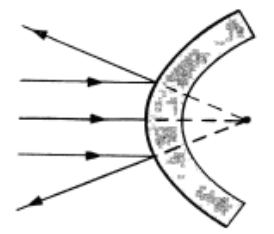
\includegraphics[scale=0.29]{fig1a}}
		\hspace{1 cm}
		\subfigure{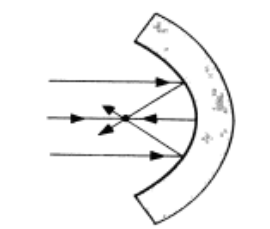
\includegraphics[scale=0.29]{fig1b}}
		\hspace{1 cm}
		\subfigure{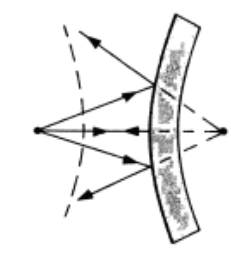
\includegraphics[scale=0.26]{fig1c}}\\
		\subfigure{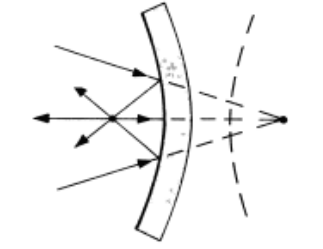
\includegraphics[scale=0.281]{fig1d}}
		\hspace{0.5 cm}
		\subfigure{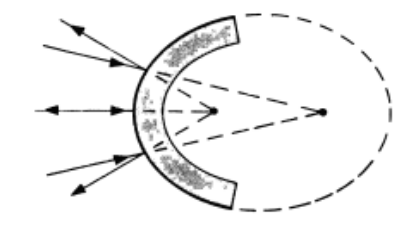
\includegraphics[scale=0.29]{fig1e}}
		\hspace{0.5 cm}
		\subfigure{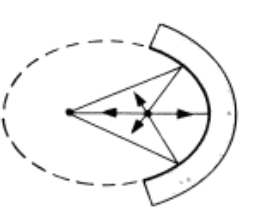
\includegraphics[scale=0.35]{fig1f}}
		\caption{{\small  {(a) Parabólico convexo. (b) Parabólico cóncavo. (c) Hiperbólico convexo. (d) Hiperbólico cóncavo (e) Elíptico convexo. (f) Elíptico cóncavo.}}}
		\label{fig:fig1}
	\end{figure*}
La ecuación paraxial que relaciona el objeto conjugado y puntos imagen con los parámetros físicos de un espejo esférico pueden deducirse de manera muy simple con la ayuda de la figura 2. Para ello notemos que  $\theta_{i}=\theta_{r}$ el $\measuredangle SAP$ es cortado en dos partes iguales por $\overline{CA}$, que por consiguiente divide al lado $\overline{SP}$ del triangulo $SAP$ en segmentos proporcionales a los dos lados restantes, esto es
\begin{equation}
\dfrac{\overline{SC}}{\overline{SA}}=\dfrac{\overline{CP}}{\overline{PA}}
\end{equation}
Además
$$\overline{SC}=s_{0}-|R|$$
y
$$\overline{CP}=|R|-s_{i}$$
donde $s_{0}$ y $s_{i}$ están a la izquierda siendo, por lo tanto, positivas. Si utilizamos la misma convención de signos que la usada comúnmente en temas de refracción, $R$ será negativa por que $C$ se halla  a la izquierda de $V$ es decir, la superficie es cóncava. 
\begin{figure}[h!]
	\centering
	\subfigure[]{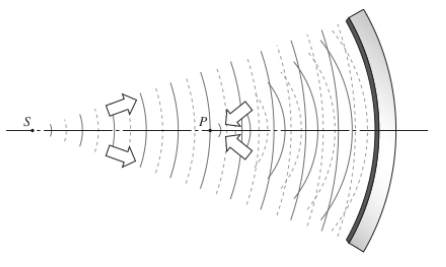
\includegraphics[scale=0.5]{fig2a}}
	\subfigure[]{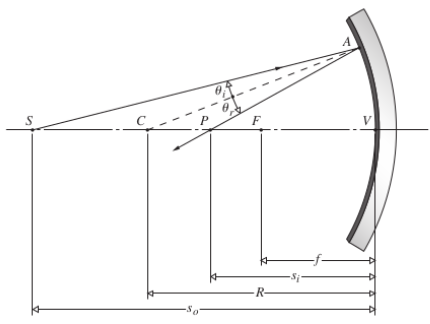
\includegraphics[scale=0.5]{fig2b}}
	\caption{Espejo esférico cóncavo. Focos conjugados }
	\label{fig:fig2}
\end{figure}
Entonces $|R|=-R$ y 
$$\overline{SC}=s_0+R$$
y $$\overline{CP}=-(s_{0}+R)$$
En la región paraxial $\overline{SA}\approx s_{0}$, y $\overline{PA}\approx s_{i}$, así la ecuación (1) queda
$$\dfrac{s_{0}+R}{s_{0}}=-\dfrac{s_{i}+R}{s_{i}}$$
o bien 
\begin{equation}
\dfrac{1}{s_{0}}+\dfrac{1}{s_{i}}=-\dfrac{2}{R}
\end{equation}
La ecuación (2) se denomina la \textbf{fórmula de los espejos}. Es aplicable tanto a espejos cóncavos $(R<0)$ como convexos $(R>0)$. El \emph{foco objeto } o \emph{primario} se define por 
$$\lim_{s_{i}\rightarrow\infty}s_{0}=f_{0}$$
mientras que el \emph{foco imagen} o \emph{secundario} corresponde a 
$$\lim_{s_{0}\rightarrow\infty}s_{i}=f_{i}$$
De la ecuación (2) se tiene que 
$$\dfrac{1}{f_{0}}+\dfrac{1}{\infty}=\dfrac{1}{\infty}+\dfrac{1}{f_{i}}=-\dfrac{2}{R}$$
Lo cual implica que
\begin{equation}
f_{0}=f_{i}=-\dfrac{R}{2}
\end{equation}
quitando los subíndices de las distancias focales se tiene que 
\begin{equation}\label{ec4}
\dfrac{1}{s_{0}}+\dfrac{1}{s_{i}}=\dfrac{1}{f}
\end{equation} 
Al igual que en lentes, se tiene que la ecuación que permite calcular el aumento lateral o magnificación es la siguiente
\begin{equation}\label{ec11}
m=-\dfrac{s_{i}}{s_{o}}
\end{equation}
}
\section*{Experimentos}
{
	Se realizó un solo experimento, solo que este experimento se dividió en dos partes, pues en la  primer parte se tomaron las medidas usando un espejo cóncavo, en la segunda parte se utilizo un espejo convexo.
	Para la primer parte experimental se realizo lo siguiente:
	\begin{itemize}
		\item [ 1.- ] Colocamos un espejo cóncavo, y seguido a este se colocó un panel. 
		\item [ 2.- ] Se vario la distancia hasta obtener una imagen nítida.
		\item [ 3.- ] Se midió la distancia de la rendija al espejo y del espejo al panel.
		\item [ 4.- ] Se midió el tamaño original de la figura y su tamaño en el panel (magnificado)
		\item [ 5.- ] Se repitieron los pasos anteriores hasta llenar la tabla 1.
	\end{itemize}
	Para la segunda parte experimental se realizo lo siguiente:
	\begin{itemize}
		\item [ 1.- ]	Se verifico primero que la imagen en la pantalla fuera nítida.
		\item [ 2.- ]	Se colocó un espejo convexo en el sitio donde debería ir el cóncavo de la parte experimental anterior.
		\item [ 3.- ]	Se colocó una lente auxiliar entre la rendija y el panel.
		\item [ 4.- ]	Se movió el espejo hasta lograr formar una imagen nítida en el panel.
		\item [ 5.- ]	Se midió la distancia del panel al espejo y de la lene al panel, los datos se registraron en la tabla 2.
	\end{itemize}
El arreglo experimental se puede apreciar en la figura 3. 
\begin{figure}[h!]
	\raggedleft
	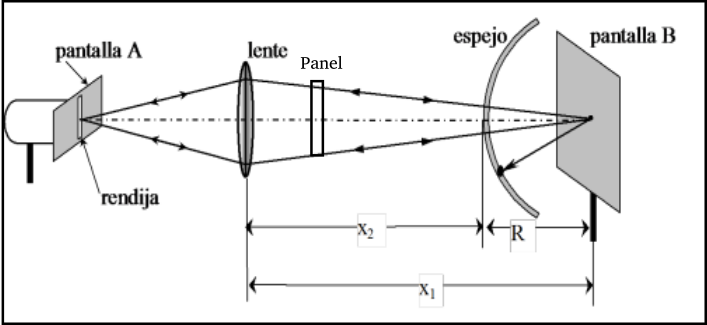
\includegraphics[width=0.9\linewidth]{fig3}
	\caption{Arreglo experimental}
	\label{fig:fig3}
\end{figure}
El arreglo experimental fue casi el mismo para ambas partes experimentales.
}
\section*{Datos obtenidos}
{
 	Los datos obtenidos para la primer parte experimental, es decir cuando los espejo era cóncavo se observan en la tabla 1, mientras que los  datos para espejos convexos se observan en la tablas 2 y 3.
 	
 	\begin{table}[htb]
 		\raggedright
 		\begin{tabular}{cccccc}
 			N & $s_{o}$ ($cm$) & $s_{i}$ ($cm$)  & $m$ & Obj & Imag  \\ \midrule
			1	&	90	&	31.9	&	-0.35	&	0.57	&	0.21	 \\
			2	&	85	&	34.4	&	-0.4	&	0.57	&	0.22	 \\
			3	&	80	&	36.6	&	-0.45	&	0.57	&	0.27	 \\
			4	&	75	&	37.2	&	-0.49	&	0.57	&	0.34	 \\
			5	&	70	&	38.4	&	-0.54	&	0.57	&	0.35	 \\
			6	&	68	&	38.4	&	-0.56	&	0.57	&	0.44	 \\
			7	&	64.9	&	49.1	&	-0.75	&	0.57	&	0.42	 \\
			8	&	55	&	44.6	&	-0.81	&	0.57	&	0.46	 \\
			9	&	52.5	&	46.2	&	-0.88	&	0.57	&	0.51	 \\\hline
 		\end{tabular}
 		\caption{Datos obtenidos en el experimento con el espejo cóncavo de $f=+250\;mm$} \label{tabla1}
 	\end{table}
 	
 	
 	\begin{table}[htb]
 			\raggedright
 		\begin{tabular}{llllll}
 			N & $s_{o}$ ($cm$) & $s_{i}$ ($cm$)  & $m$ & Obj & Imag  \\ \midrule
			1	&	-36.5	&	14.3	&	0.39	&	1.47	&	0.58  \\
			2	&	-18.7	&	10.5	&	0.56	&	0.6		&	0.44  \\
			3	&	-13.2	&	8.8		&	0.66	&	0.85	&	0.53  \\ \hline 
 		\end{tabular}
 		\caption{Datos obtenidos en el experimento con el espejo convexo de $f=+200\;mm$ } \label{tabla2}
 	\end{table}
 	\begin{table}[htb]
 		\raggedright
 	\begin{tabular}{cccccc}
 		N & $s_{o}$ ($cm$) & $s_{i}$ ($cm$)  & $m$ & Obj & Imag  \\ \midrule
 		1	&	-11.9	&	28.1	&	2.36	&	1.63	&	3.57	 \\
 		2	&	-11		&	22.1	&	2.00	&	0.9		&	1.67	 \\
 		3	&	-10.2	&	19.8	&	1.94	&	0.5		&	0.32	 \\ \hline 
 	\end{tabular}
 	\caption{Datos obtenidos en el experimento con el espejo convexo de $f=+250\;mm$} \label{tabla3}
 \end{table}
 	
}
\begin{multicols}{2}
	
	\section*{Resultados obtenidos}
	
			De la ecuación (\ref{ec4}) se tiene que 
		$$\dfrac{1}{f}=\dfrac{1}{s_{o}}+\dfrac{1}{s_{i}}$$
		proponiendo el siguiente cambio de variable 
		\begin{equation}\label{ec6}
		y=\dfrac{1}{s_{i}}\;\;\;\;\;x=\dfrac{1}{s_{o}}
		\end{equation}
		se tiene que 
		\begin{equation}\label{ec7}
		y=\dfrac{1}{f}-x
		\end{equation}
		El comportamiento grafico de los datos de la tabla 1 se muestra en la figura \ref{fig:fig-4}.  \\
		Utilizando el cambio de variable propuesto en (\ref{ec7}) se obtiene la siguiente ecuación de ajuste
		\begin{equation}
			y=0.0419-1.0874x
		\end{equation}
		La ecuación anterior implica que 
		$$f=(0.0419)^{-1}=23.86\;cm$$
		El grafico de la ecuación anterior se muestra en la figura \ref{fig:fig-5}
		\begin{Figure}
			\raggedleft
			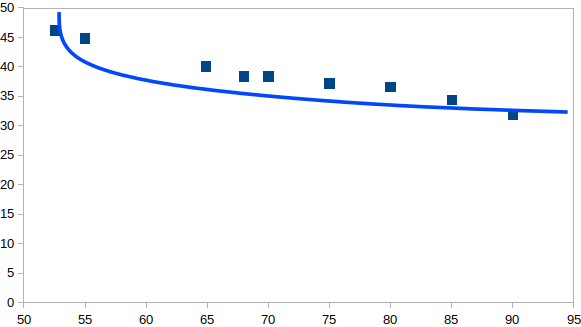
\includegraphics[width=\linewidth]{fig4}
			\captionof{\footnotesize{Grafica de los $s_{i}\;vs\;s_{o}$ datos de  la tabla \ref{tabla1}.}}
			\label{fig:fig-4}
		\end{Figure}
	\begin{Figure}
		\raggedleft
		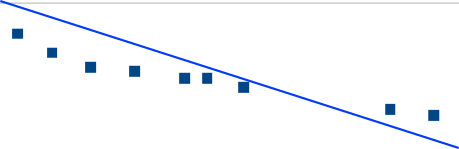
\includegraphics[width=\linewidth]{fig5}
		\captionof{\footnotesize{Grafica de los $s_{i}\;vs\;s_{o}$ datos de  la tabla \ref{tabla1} utilizando el cambio de variable (\ref{ec6}).}}
		\label{fig:fig-5}
	\end{Figure}
	El error porcentual es de 
	$$e\%=\dfrac{|25-23.86|}{25}\times 100=4.56 \%$$
	
	
	
	El comportamiento grafico de los datos de la tabla 2 se muestra en la figura \ref{fig:fig-6}.  \\
	Utilizando el cambio de variable propuesto en (\ref{ec7}) se obtiene la siguiente ecuación de ajuste
	\begin{equation}
	y=0.0456-0.9026x
	\end{equation}
	La ecuación anterior implica que 
	$$f=(0.0456)^{-1}=-21.9298\;cm$$
	El grafico de la ecuación anterior se muestra en la figura \ref{fig:fig-7}
	\begin{Figure}
		\centering
		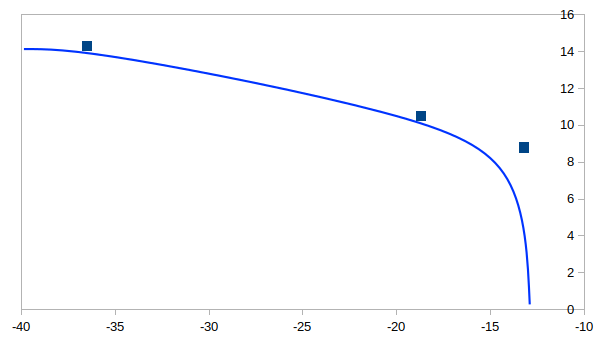
\includegraphics[width=\linewidth]{fig6}
		\captionof{\footnotesize{Grafica de los $s_{i}\;vs\;s_{o}$ datos de  la tabla \ref{tabla2}.}}
		\label{fig:fig-6}
	\end{Figure}
	\begin{Figure}
		\centering
		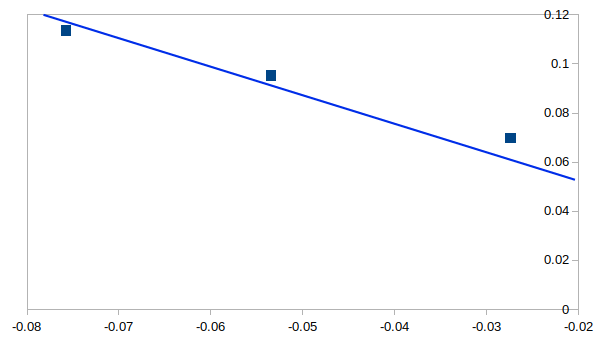
\includegraphics[width=\linewidth]{fig7}
		\captionof{\footnotesize{Grafica de los $s_{i}\;vs\;s_{o}$ datos de  la tabla \ref{tabla2} utilizando el cambio de variable (\ref{ec6}).}}
		\label{fig:fig-7}
	\end{Figure}
	El error porcentual es de 
	$$e\%=\dfrac{|-20+21.9298|}{20}\times 100 =9.64 \%$$
	
	
	El comportamiento grafico de los datos de la tabla 3 se muestra en la figura \ref{fig:fig-8}.  \\
	Utilizando el cambio de variable propuesto en (\ref{ec7}) se obtiene la siguiente ecuación de ajuste
	\begin{equation}
	y=-0.0529-1.0631x
	\end{equation}
	La ecuación anterior implica que 
	$$f=(-0.0529)^{-1}=-18.90\;cm$$
	El grafico de la ecuación anterior se muestra en la figura \ref{fig:fig-8}
	\begin{Figure}
		\centering
		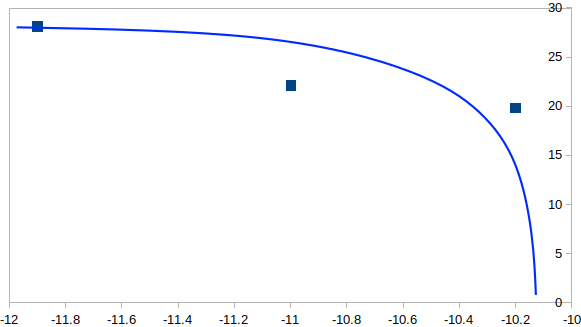
\includegraphics[width=\linewidth]{fig8}
		\captionof{\footnotesize{Grafica de los $s_{i}\;vs\;s_{o}$ datos de  la tabla \ref{tabla3}.}}
		\label{fig:fig-8}
	\end{Figure}
	\begin{Figure}
		\centering
		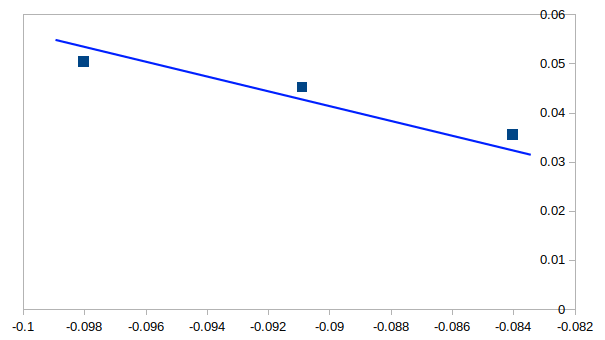
\includegraphics[width=\linewidth]{fig9}
		\captionof{\footnotesize{Grafica de los $s_{i}\;vs\;s_{o}$ datos de  la tabla \ref{tabla3} utilizando el cambio de variable (\ref{ec6}).}}
		\label{fig:fig-9}
	\end{Figure}
	El error porcentual es de 
	$$e\%=\dfrac{|-25+18.90|}{25}\times  =24.4\%$$
	
	
	\section*{Conclusiones}
	{
		De la parte con lentes espejos convexos se observa que los resultados obtenidos son buenos pues el porcentaje de error es de menos de $5\%$, por el contrario  en el caso de los espejos convexos se obtuvo un error porcentual muy elevado, esto posiblemente se deba a la pequeña cantidad de datos que se tomo para realizar el ajuste, tal vez si hubiesen sido más datos los resultados obtenidos podrían haber sido mejores.
	}
	
	
	\nocite{Hecht}\nocite{Rossi}\nocite{Sears}\nocite{Born}\nocite{Tipler}\nocite{Feynman}\nocite{Res}
	\bibliography{miBiblio.bib}
	\bibliographystyle{plain}

\end{multicols}
\end{document}
